\section{Introduction} \label{sec:introduction}

Our digitalised society and economy rely increasingly on digital services. Correspondingly, new datacenters are being built, and existing datacenters are scaled up~\cite{DBLP:journals/corr/abs-2206-03259, nicolae5377101m3sa, DBLP:conf/sc/AndreadisVMI18, market:IDC24AI}. Regarded as a state-of-the-art practice in the community, operators use simulation for designing and operating datacenters~\cite{DBLP:journals/corr/abs-2206-03259, nicolae5377101m3sa, DBLP:conf/ccgrid/MastenbroekAJLB21}, thus allowing experimentation in a time and cost-efficient way~\cite{Iosup2024DigitalTwins, DBLP:conf/ccgrid/MastenbroekAJLB21}. For example, in the European project Graph Massivizer, simulators predict speedup, failure cost, energy consumption, and CO2 emissions for massive-scale infrastructure~\cite{nicolae5377101m3sa, DBLP:conf/compsac/MolanKBTPCIRRVP23, DBLP:conf/wosp/IosupPVTMHZBFK23, DBLP:conf/wosp/Sanchez0RP23}. Simulating massive-scale distributed computer ecosystems under workload is a critical, yet non-trivial task due to the peculiar behaviour of various hardware and software layers of the ecosystem when under operational phenomena~\cite{DBLP:conf/wosp/ChuTVI23, DBLP:conf/ccgrid/KondoJIE10}; addressing this challenge, multiple simulators have been proposed over the past decades, such as the open-source OpenDC~\cite{DBLP:conf/ccgrid/MastenbroekAJLB21}, Kavier~\cite{Nicolae2025BSc}, CloudSim~\cite{DBLP:journals/spe/CalheirosRBRB11}, or DCSim~\cite{DBLP:conf/cnsm/TigheKBL12}. 
Although existing simulators are still valuable for simulating datacenters under workload, in ICT, there is currently no closed-loop operational ecosystem adopting a physical-digital-twinning workflow that continuously ingests live telemetry, updates the digital twin, and actuates the physical infrastructure based on SLO-aware simulation feedback. To address this operational gap, datacenter operators manually intervene or adopt static thresholds, often resulting in delayed and inefficient decisions, cascading into violations of Service Level Objective (SLO) and low Quality of Service (QoS)~\citationsneeded{2}. Addressing this gap, in this work, we design, prototype, and evaluate \underline{OpenDT}, the first \underline{Open}-source \underline{D}igital \underline{T}winning operational ecosystem for datacenters.

\Cref{fig:high-level-element} illustrates a high-level design of OpenDT, which involves continuous communication between a physical twin (left) and a digital twin (right), adapted with permission from~\cite{Iosup2024DigitalTwins}. The physical twin collects telemetry data and communicates with the digital twin, which, through simulation-based and SLO-oriented analysis, steers the physical ICT infrastructure. 



\begin{figure}
    \centering
    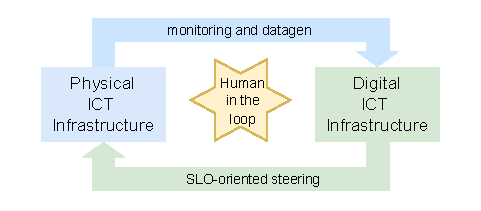
\includegraphics[width=0.98\linewidth]{report/figures/high-level-overview-dt-pt.pdf}
    \vspace*{-0.2cm}
    \caption{High-level overview of datacenter digital twinning system. The Physical ICT infrastructure collects telemetry data and directs it to the Digital ICT infrastructure, which, through simulation, offers back adjustment feedback best-aligned with the active SLOs. A human in the loop oversees the process and ensures the correctness and ethicality of the process. Adapted with permission from~\cite{Iosup2024DigitalTwins}.}
    \label{fig:high-level-element}

    \vspace*{-0.7cm}
\end{figure}

% \begin{itemize}
%     \item A data-driven digital shadow of a SURF datacenter that replays real workloads, visualizes power \& CO$_2$, and proposes simulation-based mitigations when issues arise.
%     \item Datacenter-level view (scheduler $\rightarrow$ nodes $\rightarrow$ jobs), representing how tasks are placed and executed across CPU/GPU nodes.
%     \item Public SURF traces (jobs + node telemetry) with timestamps enabling time-aligned replay; dataset available on Zenodo.
%     \item Simulation for decision support, ``what-if'' scenarios for failures, overloads, or carbon-aware scheduling (e.g., rescheduling a hot rack, delaying non-urgent jobs to lower-CO$_2$ windows, or shifting CPU/GPU placement) \textcolor{red}{TBD}
%     \item Understand how the real datacenter manages tasks over time, reduce energy/CO$_2$, and improve resilience
%     \item Use ML to forecast near-term load/power and CO$_2$, detect anomalies or impending failures, or recommend carbon-aware scheduling actions that cut energy and improve resilience. \textcolor{red}{TBD}
% \end{itemize}

Digital twinning ICT infrastructure is a novelty in computer systems and is innovative beyond the science of computer systems. However, in large-scale sciences such as aviation and space exploration, digital twins have been successfully used for decades, providing course-grained and dynamic adjustment the physical twin (e.g., airplanes, spaceships), from a distance, without physical access to the physical twin, yet only with operational access to the physical twin for dynamic adjustments aided by simulators coupled with live telemetry~\citationsneeded{3}. In small-scale sciences, such as applied biomedicine in cardiovascular health, digital twinning (eco)systems use patient-specific live telemetry (e.g., fusing imaging (e.g., MRI, CT), biosignals (e.g., ECG, electrocardiographic imaging)), and detailed physics-based electrophysiology simulation to predict treatment. ~\cite{sel2024building}. In contrast, to adopt a digital twinning operational ecosystem for complex datacenter ecosystems, medium-scale telemetry and models must combine higher-level abstraction with detailed monitoring and operational models for specific devices, applications, while addressing various operational phenomena~\cite{nicolae5377101m3sa}. This is fundamentally different from other-scale sciences~\cite{allen2019hierarchy, nicolae5377101m3sa}.

In this work, we address the open challenge of \textit{monitoring and operating massive-scale computer ecosystems through digital twinning}, by designing OpenDT, a first-of-its-kind ecosystem for datacenter digital twinning, implementing a prototype of the scientific instrument, and evaluating with realistic, trace-based experimentation scenarios. Adhering to the community-vetted, state-of-the-art AtLarge vision on researching distributed systems and ecosystems~\cite{iosup2019atlarge}, this paper contains a three-fold contribution:


% \todoall{There is currently no reference architecture of a digital twin. This is an issue: an ecosystem for distributed computer ecosystems can only be rigorously designed if it can be mapped to an existent, preferably also peer-reviewed, reference architecture... We can also play "the scientist" game, but this design otherwise is not robust science...}

\begin{enumerate}[label=\textbf{C\arabic*}]
\item \label{introduction:c1} (\textbf{Design}) We design OpenDT (steps 1-4 from \cite{iosup2019atlarge}, the first \underline{open}-source operational ecosystem for \underline{d}igital \underline{t}winning datacenters (\Cref{sec:design}). We formulate functional and non-functional requirements, then analyze design choices of OpenDT against the established requirements. We further the design of OpenDT and propose an operational workflow for the digital twinning ecosystem. We design the simulator component as generic, integrable with discrete-event simulators. Overall, OpenDT is modular and allows for each component to have various internal designs and implementations.

\item \label{introduction:c2} (\textbf{Prototype and experimentation}) 
We prototype OpenDT in \Cref{sec:prototype} (step 5 from \cite{iosup2019atlarge}). For the simulation component, OpenDT integrates OpenDC~\cite{DBLP:conf/ccgrid/MastenbroekAJLB21}, a peer-reviewed, state-of-the-art datacenter simulator, with over 8 years of operational experience and employed in national-scale projects (e.g., 6G Future Network Services~\cite{FutureNetworkServices2025}) and European-scale projects (e.g., Graph Massivizer~\cite{GraphMassivizer2025}). 
% Then, in \Cref{sec:experiments}, we conduct three experiments (step 6 and 7~\cite{iosup2019atlarge}) aided by OpenDT to: (i) exp 1 (maybe show a real-world scenario and how digital twinning be better than just simulation), (ii) exp 2 (tbd), (iii) exp 3 (tbd). 
Overall, OpenDT enables...
operators
+ researchers
+ students
% \todoall{add findings here}.
% \todoall{actually make this capsule and add the link here.}


\end{enumerate}
 



